\section{Deep Learning Methods in Action Recognition}
META: Review of approaches that use Deep Learning.

\subsection{Spatio-Temporal Networks}
I.e. convolutional methods.

\subsubsection{3D Convolutional Neural Networks for Human Action Recognition -- Ji et al. (2010/2013)}
NOTE:Paper was first published in 2010, the publication of 2013 is more popular however.

In this work \cite{ji_3d_2013} the authors porpose 3D convolution for action recognition from video, which processes spatial as well as temporal information in a convolutional layer.

In regular convolutional neural networks 2D convolutions are applied in the convolutional layers to extract features from the feature maps in the previous layer. More formally in the notation of the authors, the value of feature map $j$ in the $i$th layer at spatial position $(x,y)$ is given by:

\begin{align*}
    v_{ij}^{xy} = \tanh \left( b_{ij} + \sum_m \sum_{p=0}^{P_i -1} \sum_{q = 0}^{Q_i - 1} w_{ijm}^{pq} v_{(i-1)m}^{(x+p)(y+q)} \right)
\end{align*}

$w_{ijm}^{pq}$ denotes the value at position $(p,q)$ of the kernel, that performs convolution on feature map $m$ of the previous layer, resulting in feature map $j$ in layer $i$.
$P_i$ and $Q_i$ denote the dimensions of the kernel in x- and y-direction respectively.
Tensor $w$ therefore represents all kernels that produce the feature maps in layer $i$ through convolution.

The two inner sums carry out the convolutional operation on feature map $m$ of the previous layer, which is then combined with the results for the other feature maps by summation over $m$, added with a bias and fed into a non-linear function ($\tanh(\cdot)$) to result in the value of the current feature map.

Note: The convolutional operation used here is called cross-correlation, which differs from mathematical discrete convolutions in that the kernel is not flipped. This results in a non-commutative operation as described in chapter 9 of cite deep learning book ??

The authors propose an extension of 2D convolutions by using a three dimensional kernel. More formally, in the notation as above, the value of feature map $j$ in the $i$th layer at position $(x,y,z)$ is given by:

\begin{align*}
    v_{ij}^{xyz} = \tanh \left( b_{ij} + \sum_m \sum_{p=0}^{P_i -1} \sum_{q = 0}^{Q_i - 1} \sum_{r = 0}^{R_i - 1} w_{ijm}^{pqr} v_{(i-1)m}^{(x+p)(y+q)(z+r)} \right)
\end{align*}

As above, $w_{ijm}^{pqr}$ denotes the value of the now three dimensional kernel at position $(p,q,r)$, which performs convolution on the $m$th feature map of the previous layer.
$R_i$ denotes the dimension of the kernel in temporal direction. 

Based on the 3D convolution, the authors design a neural network architecture, that takes an input of 7 frames of size 60x40.

The network is evaluated as part of an action detection and recognition system on the TRECVID (TREC Video Retrieval Evaluation) data, which consists of surveillance videos recorded at London Gatwick Airport.

The details of the architecture are described below:

\begin{figure}[H]
    \centering
    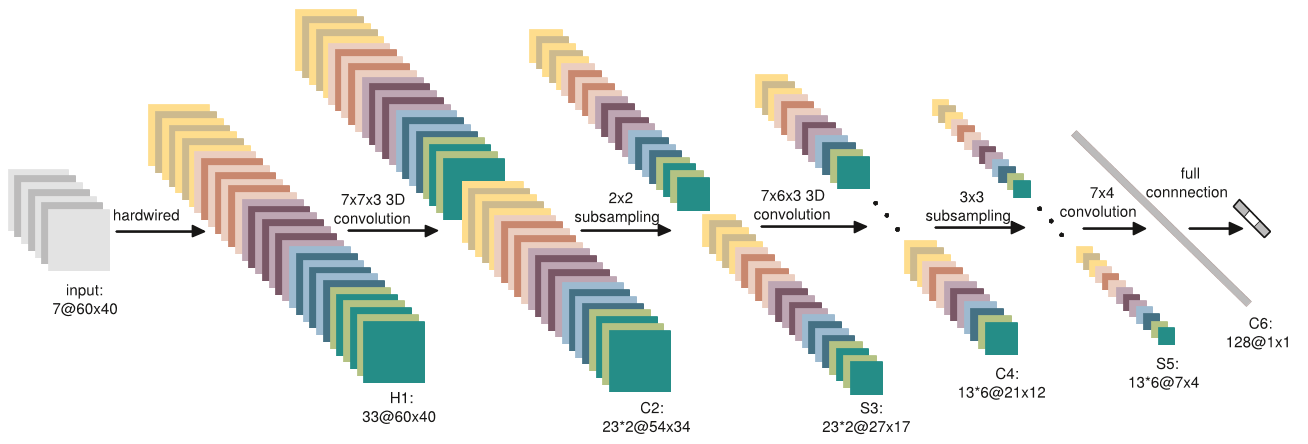
\includegraphics[width=\textwidth]{img_deep/3dconv_architecture}
    \caption{3D CNN architecture developed for human action recognition on the TRECVID 2008 development dataset \cite{ji_3d_2013}}
    \label{fig:3dconv_architecture}
\end{figure}

At first, hard wired kernels are applied to the input frames, which extract gray values, gradients along the horizontal and vertical direction in the frames and the optical flow between two consecutive frames. This results in 33 feature maps, organized in 5 different channels: gray, gradient-x, gradient-y, optflow-x and optflow-y.

In the first convolutional layer (C2) two 3D kernels with dimesions 7x7x3 (7x7 in the spatial dimension and 3 in the temporal dimension) are applied at each of the five channels separately. 
This results in 2x5 channels with a total of 46 feature maps.
The first convolutional layer therefore necessitates $2 \times 5 \times 7 \times 7 \times 3 \text{ (kernel-weights) } + 2 \times 5 \text{ (biases) } = 1480$ trainable parameters. 

After subsampling layer S3, three different kernels with size 7x7x3 are applied to each of the 2x5 channels of the previous layer.

The last convolutional layer then performs, after 3x3 subsampling, 2D convolutions to obtain 128 feature maps of dimension 1x1.
These feature maps can be seen as a 128 dimensional feature-vector representation of the input.

The resulting feature-vector is classified by a fully connected layer (into three different classes).

The architecture has 295.458 trainable parameters in total, which are initialized randomly and learned by online error back-propagation as in cite lecun 1998 ??.
NOTE: Perhaps add comparison to recent image recognition networks here. ??

The authors tried other layouts but conclude that the one described above works best. The performance was evaluated on the TRECVID 2008 development dataset ?? and on the KTH dataset ??.

\textbf{TRECVID:}\\
The TRECVID 2008 development dataset contains 49-hour annotated surveillance videos from five different cameras on five days.
The authors train their model to recognize three different action classes from the dataset: CellToEar, ObjectPut and Pointing.
The other classes were used to generate negative training examples.

\begin{figure}[H]
    \centering
    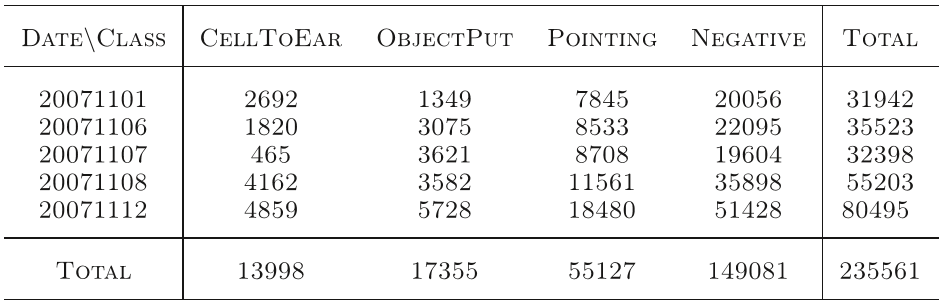
\includegraphics[width=0.75\textwidth]{img_deep/3dconv_dataset}
    \caption{Number of samples per class from the TRECVID 2008 development dataset \cite{ji_3d_2013}}
    \label{fig:3dconv_dataset}
\end{figure}

Since the dataset provides continuous videos with several persons in a real-world scence, the authors apply a human detector and a detection-driven tracker, to keep track of the heads in the scene.
This information is used to extract a bounding box around a person, as soon as an action is performed. 
Six other equally sized bounding boxes are sampled at the same location from three frames before and after the intial frame.
Between those samples, one frame is omitted which results in a temporal step size of 2.

The contents of these 7 bounding boxes are stacked and taken as input to the 3D CNN architecture for classification.

\begin{figure}[H]
    \centering
    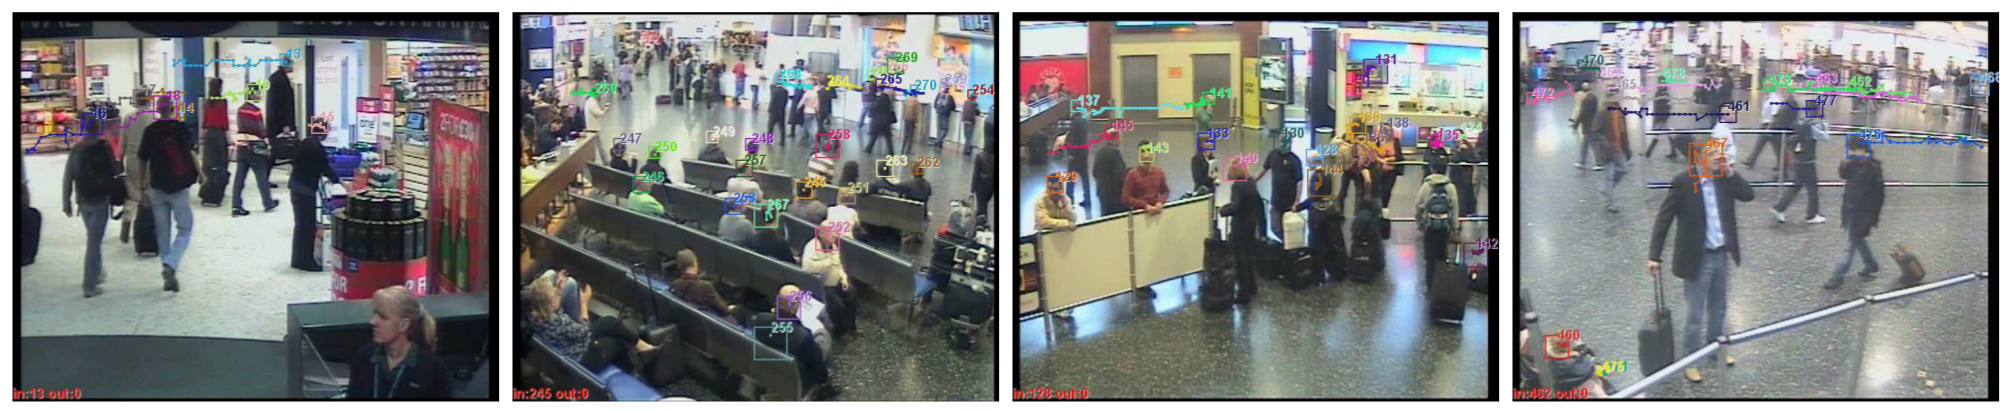
\includegraphics[width=\textwidth]{img_deep/3dconv_sampletracking}
    \caption{Example scenes taken by different cameras with the results of the human detection and tracking \cite{ji_3d_2013}}
    \label{fig:3dconv_sampletracking}
\end{figure}

In order to compare their 3D CNN model to other techniques, the authors also evaluate:
\begin{enumerate}
    \item A frame based 2D CNN model
    \item Extraction of dense SIFT features from the gray images of the 3D CNN input cube, which are then aggregated using the BoW-Paradigm and classified through a linear SVM
    \item Extraction of dense SIFT features from the motion edge history images (MEHI) of the 3D CNN input cube, which are then aggregated as above.
\end{enumerate}

The 3D CNN model outperfomed the other approaches on the TRECVID 2008 development dataset on all classes except Pointing, where the 2D frame-based CNN performed best.
The authors note, that the positive example for Pointing are significantly larger than for the other classes and conclude, that their architecture performs best, when little positive examples are present.

\textbf{KTH:}\\
Additionally, the 3D CNN model was evaluated on the KTH dataset.
It achieves an overall accuracy of 90.2\%.

DISCUSSION: Authors cite the work of schindler and van gool from 2008 and state, that 5-7 frames are enough for action recognition.
Schindler and van gool: 5-7 frames are enough to recognize SIMPLE actions.

\subsubsection{Sequential Deep Learning for Human Action Recognition -- Baccouche et al. (2011)}
\textcite{baccouche_sequential_2011} identify two issues with the previous approaches for extending convolutional neural networks to the video domain, i.e. 3D convolutions as in \cite{ji_3d_2013} and \cite{kim_human_2007}:

\begin{enumerate}
    \item They rely on hand crafted inputs (hard wired preprocessing of the data to produce image gradients or optical flow in the first processing layer).
    \item The models typically process less than 15 input frames, and therefore only classify short sub-clips, not the entire video.
\end{enumerate}

To address these issues, the authors design a two-step deep architecture consisting of:

\begin{enumerate}
    \item A convolutional spatio-temporal feature extractor network, based on 3D convolutions.
    \item A recurrent neural network classifier, that incorporates LSTM cells \cite{hochreiter_long_1997}, to classify the entire sequence of previously extracted spatio-temporal features.
\end{enumerate}

The architecture is trained and evaluated on the KTH dataset.

\begin{figure}[H]
    \centering
    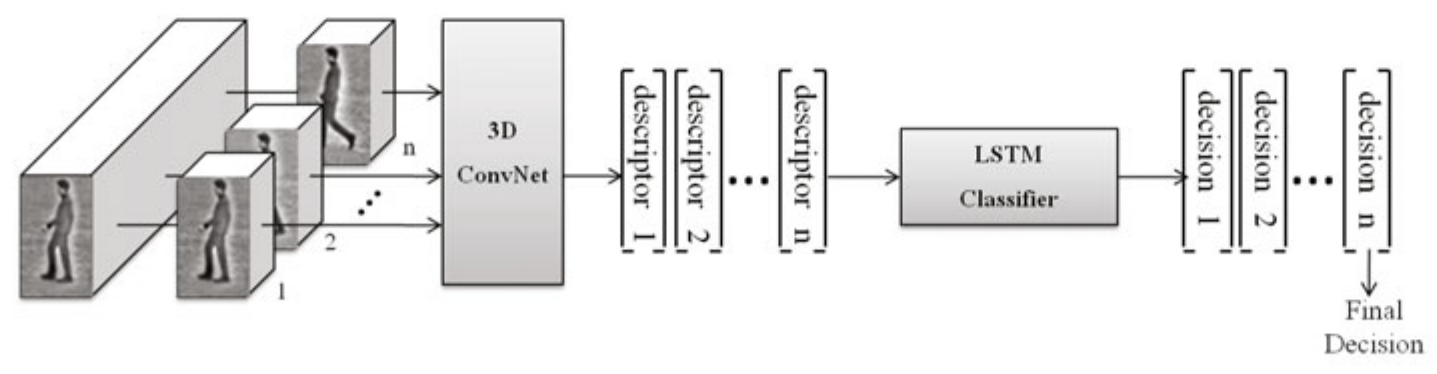
\includegraphics[width=\textwidth]{img_deep/sequentialdeep_overview.png}
    \caption{Overview of the two-steps architecture consisting of a 3D ConvNet and a RNN classifier. \cite{baccouche_sequential_2011}}
    \label{fig:sequentialdeep_overview}
\end{figure}

The ConvNet architecture of this approach is depicted in figure \ref{fig:sequentialdeep_overview}.
It is comparable to the one of \textcite{ji_3d_2013} in that it incorporates 3D convolutions, but works on raw input pixels instead of hand-crafted inputs.

\begin{figure}[H]
    \centering
    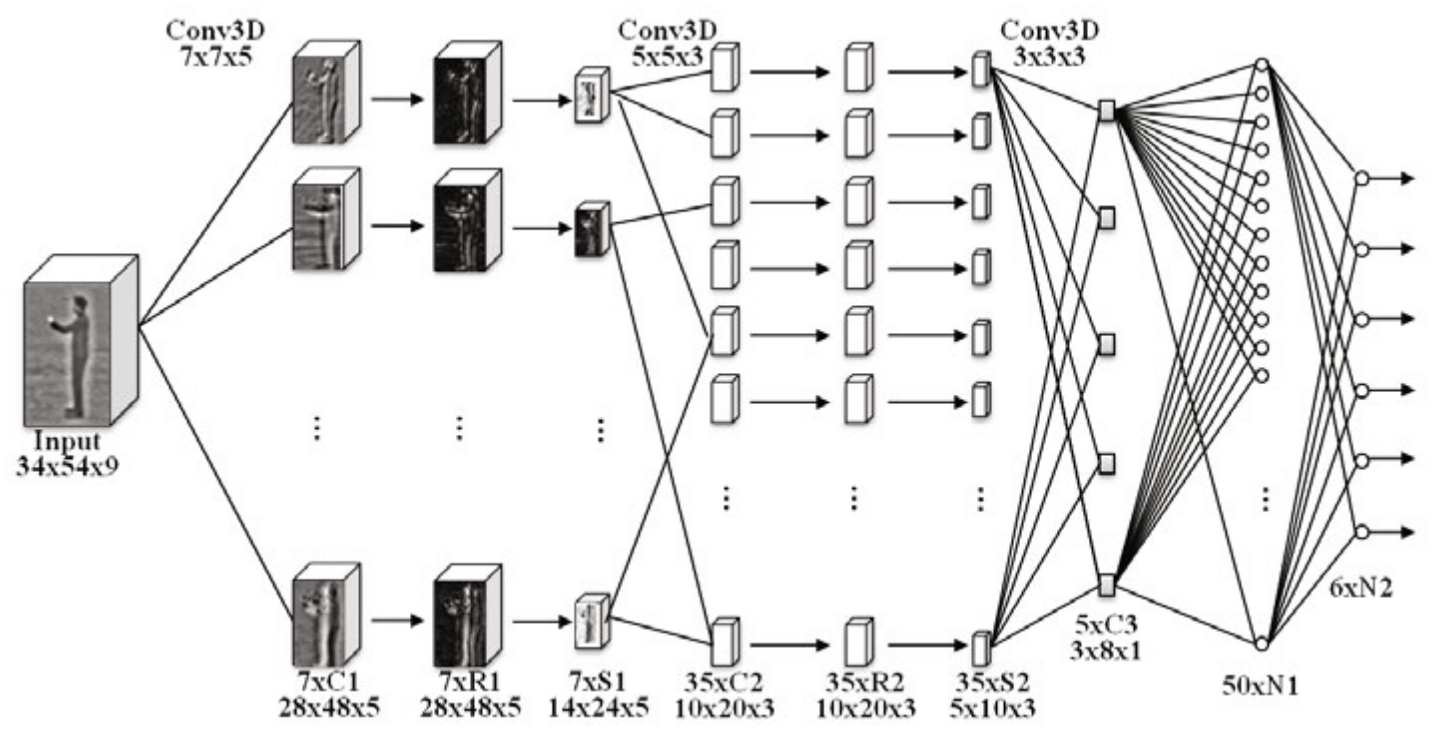
\includegraphics[width=0.9\textwidth]{img_deep/sequentialdeep_cnnarchitecture}
    \caption{3D ConvNet architecture for the extraction of spatio-temporal features \cite{baccouche_sequential_2011}}
    \label{fig:sequentialdeep_cnnarchitecture}
\end{figure}

Input to the network is formed by stacking 9 succesive frames of spatial size 34x54, which results in an input cube of dimension 34x54x9.

The configuration of it's layers is as follows:

\begin{enumerate}
    \item First convolutional layers C1 computes 7 feature maps, by convolving a 3D 7x7x5 kernel for each feature map with the input cube.
    \item Layer R1 and S1 perform rectification (building of the absolute value) and subsampling with a spatial factor of 2 respectively.
    \item Second convolutional layer C2 computes 35 feature maps. Each of the 7 feature maps in layer S1 is connected to two different feature maps in C2 (resulting in 14 feature maps) and each pair of different feature maps of S1 is connected to one feature map in C2 (resulting in additional 21 feature maps, leaving a total of 35 feature maps).
    \item Layer R1 and S2 are equivalent to R1 and S1.
    \item Third (and last) convolutional layer C3 computes five features maps, which are fully connected to all feature maps in previous layer S2 by 3x3x3 kernels. These five feature maps have dimension 3x8x1, rendering the raw input encoded into a 120 dimensional feature vector.
    \item For training the individual ConvNet model, the 120D feature vector is finally fed into two fully connected layers with 6 output neurons (one for each class of the KTH dataset).
\end{enumerate}

The ConvNet model embeds a total of 17,169 trainable parameters, which is about 15 times less than the number of parameters trained by \textcite{ji_3d_2013} (295,458 parameters).

The authors use the same training algorithm as Ji et al., which was proposed by cite lecun 1998 ??: online Backpropagation with momentum adapted to weight-sharing.

In order to take the temporal evolution of movements in a video into account, the authors propose to train a recurrent neural network with one hidden layer of LSTM cells for classifying sequences of previously extracted CNN feature-vector representations.

Several configurations were tested and 50 LSTM cells in the hidden layer were found to be a good compromise between training time and performance.

The output of the third convolutional layer C3 of the ConvNet architecture is fed into the recurrent neural network as input at each time step.

The LSTM cells in the hidden layer are fully connected with the input and have recurrent connections among each other. 

The output layer is connected to the outputs of the LSTM cells.

The RNN is trained as part of the two-step architecture using online backpropagation through time with momentum.

The architecture is evaluated on the KTH dataset. To build the inputs to the network, the following simple pre-processing steps are applied: down-sampling by a factor of 2 horizontally and vertically, extraction of the bounding boxes around persons, application of 3D Local Contrast Normalization on a 7x7x7 neigbourhoood.

The authors find the 3D ConvNet model to yield a recognition rate of 91.04\%, when the classification is done by majority voting over several short sub-sequences of the test-video (without using the LSTM classifier).
Which is comparable to other deep learning approaches at that time and almost the same result as obtained by \textcite{ji_3d_2013} (90.2\%), although the model requires about 15 times less paramerters.

When using the LSTM classifier network, performance increases of about 3\%. The combined two-steps architecture consistently outperformed other deep models at that time.

Evaluation scheme: five best results averages over 30 trials.

\subsubsection{Large-scale Video Classification with Convolutional Neural Networks -- Karpathy et al. (2014)}

The author's contribution in \cite{karpathy_large-scale_2014} is four-fold:
\begin{enumerate}
    \item They gather the Sports-1M dataset containing a collection of 1 million automatically annotated sports videos from YouTube.
    \item They study multiple approaches for extending convolutional neural networks to incorporate spatio-temporal information.
    \item They propose a multiresolution convolutional architecture with the goal of speeding up the training at no cost in accuracy.
    \item They retrain the top layers of a network on the UCF-101 dataset, which has previously been trained on the Sports-1M dataset and thereby achieve significant increase in performance towards training the network on UCF-101 alone (transfer learning).
\end{enumerate}

Here, the architectures will be reviewed (contributions 2. and 3.), for a description and review of the Sports-1M dataset and the transfer learning paradigm see section \ref{chap:datasets} of this work.

To obtain fixed-sized inputs for their architectures, the authors interpret an entire video as a set of short, fixed-sized video clips.

The authors first implement a baseline CNN architecture to classify videos based on a single frame.
The model is similar to the winning network of the 2012 ImageNet Classification Challenge cite ??, but receives slightly smaller inputs (here 170x170x3 against 224x224x3 in the ImageNet model).

Based on the single frame architecture, several extensions for processing temporal information in the network are being investigated. These types of fusion methods are depicted in figure \ref{fig:largescale_fusionmethods}.

\begin{figure}[H]
    \centering
    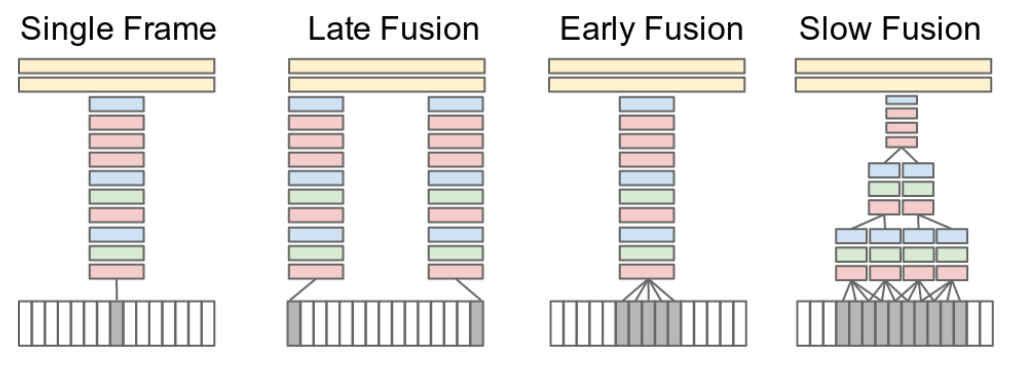
\includegraphics[width=0.75\textwidth]{img_deep/largescale_fusionmethods}
    \caption{Different methods for fusing temporal with spatial information in convolutional neural network architectures. Red, green and blue denotes convolutional, normalization and pooling-layers. Grey colored inputs are single video frames. \cite{karpathy_large-scale_2014}}
    \label{fig:largescale_fusionmethods}
\end{figure}

\textbf{Early Fusion:} \\
Temporal information is incorporated in the network on the pixel level by extending the convolutional kernel in the first layer to be of dimension $11 \times 11 \times 3 \times T$, where T is the temporal extend (here used: $T = 10$).

\textbf{Late Fusion:} \\
Two separate single-frame networks with shared parameters and without their individual classification layers are used on input frames with a temporal distance of 15 frames.
Two shared fully connected layers then merge the individual network's information and classify the input. 
The fully connected layers are able to compute motion information by comparing the feature representations of the two single-frame networks.

\textbf{Slow Fusion:} \\
Temporal information is processed throughout the network by extending the kernels of each convolutional layer in time, as done in the first layer of the Early Fusion approach.
Thereby higher layers progressively processes more spatio-temporal information of the input frames.
These kinds of convolutions have also been applied in \cite{ji_3d_2013} and baccouche ??.
The first convolutional layer uses a temporal extend of $T = 4$, while the second convolutional layer uses a temporal extend of $T = 2$, which allows the third layer to access the information of all 10 input frames.

Since the training time of a network heavily influences the amount of experiments that can be conducted on different hyperparameter settings, it is of great interest to reduce the training time for neural networks (for CNNs: in the order of weeks) while maintaining the accuracy.

The authors propose a multiresolution architecture as shown in figure \ref{fig:largescale_multiresolution}.

\begin{figure}[H]
    \centering
    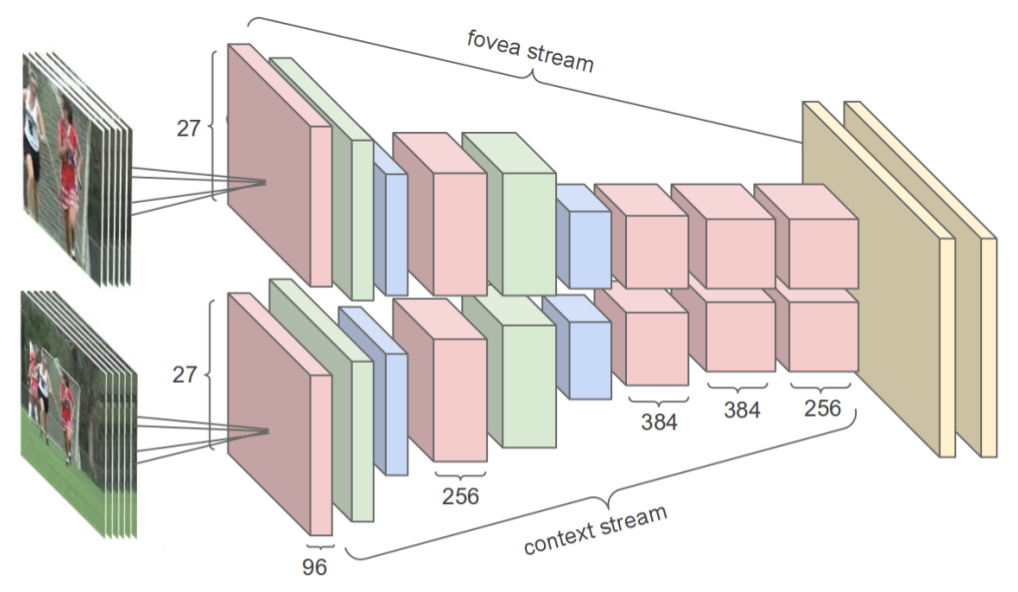
\includegraphics[width=0.75\textwidth]{img_deep/largescale_multiresolution.png}
    \caption{Multiresolution CNN architecture \cite{karpathy_large-scale_2014}}
    \label{fig:largescale_multiresolution}
\end{figure}

The overall multi-resolution network processes videos of size 178x178 pixel as input.

The context stream receives a downsampled version of the input frames, which has half the size of the original input (89x89 pixel).
The fovea stream works on just the 89x89 pixel sized center of the original input frames.

Both streams are implemented as the same CNN architecture.

The outputs of both streams are fed into the first of two fully connected layers, where their information is merged and a class prediction is calculated.

The multiresolution architecture recquires half the input dimensionality compared to processing the raw 178x178 pixel input video in one stream.

Thereby the authors achieved a reduction in training time by a factor of 2-4.

The authors use downpour stochastic gradient descent cite ?? for training the networks on the Sports-1M dataset using a computing cluster.
70\% of the dataset were used as training data, 10\% as the validation set and 20\% as the test set.

At testing time, 20 short clips are sampled from the current test-video and each clip is presented to the network individually.
Each clip is passed through the network 4 times (with different crops and flips) and the result is averaged to produce a robust class prediction.
The video-level predictions are computed from the clip-level predictions simply by averaging.

In addition to comparing different CNN architectures, the authors also implement a feature-histogram baseline approach by extracting multiple kinds of hand-crafted features from each video and aggregating them according to the bag-of-words paradigm.
The resulting feature vector is classified using multilayer neural network, with rectified linear activation units.

The performance of the studied architectures is shown in table \ref{tab:largescale_results}:

\begin{table}
    \centering
    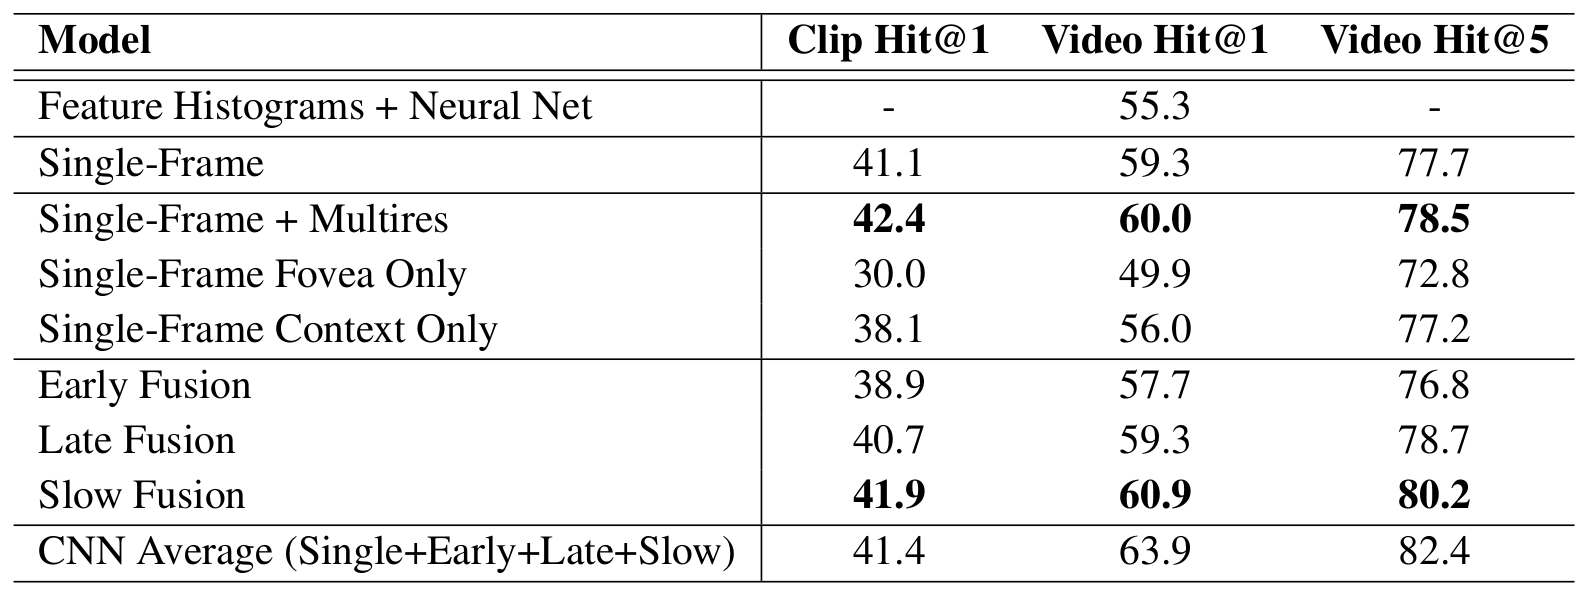
\includegraphics{img_deep/largescale_results}
    \caption{Results of different architectures on the Sports-1M dataset. Hit@$k$ denotes the fraction of test samples, that had at least one of their class labels included in the top $k$ predictions. \cite{karpathy_large-scale_2014}}
    \label{tab:largescale_results}
\end{table}

The authors find their deep models to consistently outperform the hand-crafted feature based baseline.

Compared to each other, the deep models performed similarly well, despite their different convolutional architectures. The slow fusion model however performed best, by a small margin.

According to the authors interpretation, the ``variation among different CNN architectures turns out to be surprisingly insignificant''\cite{karpathy_large-scale_2014}.

The single-frame model performs noticably well on it's own. The authors suspect, that the motion aware networks suffer from camera movements such as translations or zoom.

``we find that a single-frame model already displays very strong performance, suggesting that local motion cues may not be critically important, even for a dynamic dataset such as Sports. An alternative theory is that more careful treatment of camera motion may be necessary (for example by extracting features in the local coordinate system of a tracked point, as seen in [25]).''

\subsubsection{Learning Spatiotemporal Features with 3D Convolutional Networks -- Tran et al. (2015)}

\subsubsection{Long-term Temporal Convolutions for Action Recognition -- Varol et al. (2016)}
%Extensions of CNNs to action recognition in video have been proposed in several
%recent works [6, 12, 13]. Such methods, however, currently show only moderate
%improvements over earlier methods using hand-crafted video features [5].

\textcite{varol_long-term_2016} address, similar to \textcite{baccouche_sequential_2011}, the common drawback of recent CNN extensions to action recognition, that class labels are learned for very short video subsequences only, i.e.\ a temporal extend of only 1-16 input frames can be processed by the architectures at a time.\cite{ji_3d_2013}\cite{karpathy_large-scale_2014}\cite{tran_learning_2015}

Instead of classifying convolutionally extracted spatio-temporal features with a recurrent neural network, which is able to take their temporal evolution into account (as done by \textcite{baccouche_sequential_2011}), the authors of this publication study the effects of increasing the number of input frames of a 3D convolutional architecture on the performance in action recognition.

The authors name their approach long-term temporal convolutions. Their contribution in this work is two-fold:
\begin{enumerate}
    \item Systematical evaluation of the influence of the temporal extend, i.e.\ the number of input frames $T = \{20, 40, 60, 80, 100\}$, to the performance of a 3D CNN architecture for video action recognition.  
    \item Confirming the importance of high-quality optical flow inputs, in order to learn accurate video features with a 3D CNN architecture for human action recognition.
\end{enumerate}

Processing an increased temporal extend has to be compensated with a decreased spatial resolution, in order to not exceed computational limitations.
The studied architectures therefore process spatial resolutions of 58x58 or 71x71 pixels.

The authors' 3D CNN architecture, for which different temporal extends are studied, is shown in figure \ref{fig:longterm_architecture}.

\begin{figure}[H]
    \centering
    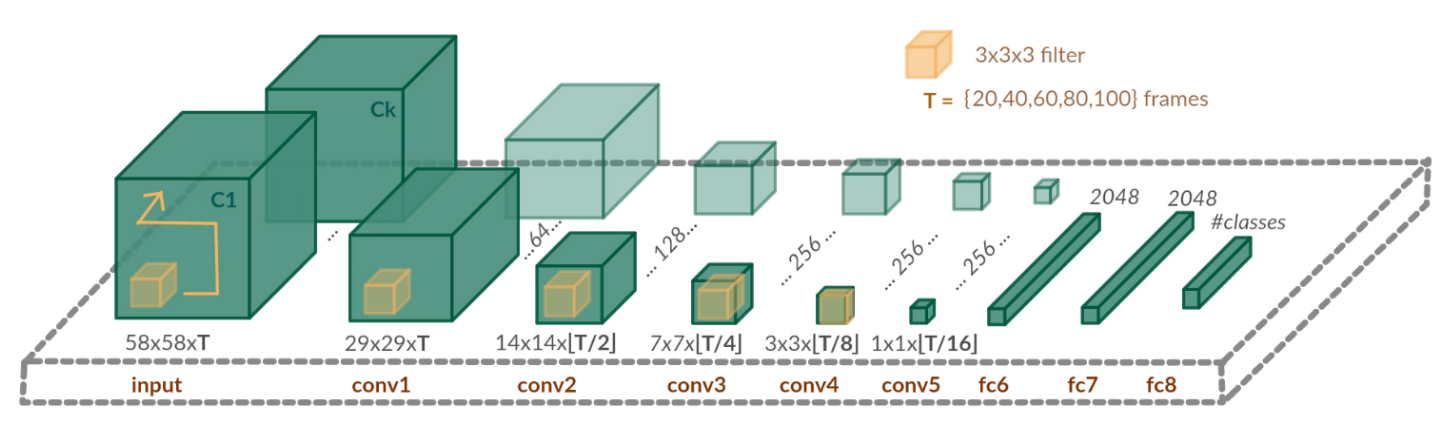
\includegraphics[width=\textwidth]{img_deep/longterm_architecture}
    \caption{3D CNN architecture for evaluating the influence of temporal extend on action recognition performance. \cite{varol_long-term_2016}}
    \label{fig:longterm_architecture}
\end{figure}

Architectural details:

\begin{itemize}
    \item 5 space-time, i.e.\ 3D, convolutional layers with 64, 128, 256, 256 and 256 feature maps.
    \item 3x3x3 space-time convolutional kernels are used in every convolutional layer.
    \item After each convolutional layer: One layer of rectified linear units (ReLU) and one layer of max-pooling with filter size 2x2x2 except in the first layer where it is 2x2x1.
    \item 3 fully connected layers at the end with sizes 2048, 2048 and number of classes.
\end{itemize}

As a baseline approach the authors implement their architecture with inputs of size 112x112x16, beacause it can directly be compared to the work of \cite{tran_learning_2015}.
Initially, the authors study the performance between the 16 frame baseline and another 60 frame network, which takes inputs of size 58x58x60 (spatial size has to be decreased to remain computationally tractable).

To systematically investigate the influence of temporal extend on the action recognition performance, the authors implement their architecture with different numbers of input frames $T = \{20, 40, 60, 80, 100\}$ and different spatial resolutions ${58 \times 58, 71 \times 71}$.

Additionally the influence of using optical flow inputs on the performance, specifically the influence of different sources of optical flow, is evaluated. These namely are:
\begin{enumerate}
    \item MPEG flow, which directly can be obtained from the video encoding. It is a fast alternative to regular optical flow estimators, but has low spatial resolution and is not available for all video frames.
    \item Farneback optical flow estimator cite ??, which is fast, but calculates noisy flow fields.
    \item Brox optical flow estimator cite ??, which generates highest quality optical flow fields but is slower than the other two methods.
\end{enumerate}

\begin{figure}[H]
    \centering
    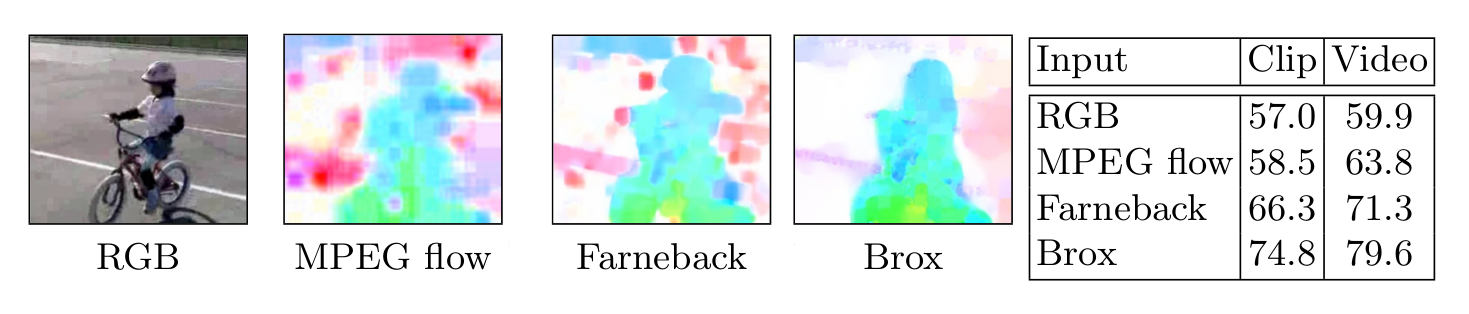
\includegraphics[width=\textwidth]{img_deep/longterm_optflow}
    \caption{You really need to add a caption here!}
    \label{fig:longterm_optflow}
\end{figure}

The networks are trained on the UCF-101 and HMDB-51 dataset using stochastic gradient descent with negative log-likelihood criterion.

During training the authors randomly sample video subsequences with the desired spatial and temporal dimensions from the input videos, which in general have a higher resolution and are longer than needed. The authors name this form of pre-processing random clipping.

Another method used during training is called multiscale cropping.
Smaller input volumes as needed are cropped from the training videos and then rescaled to fit to the input dimensions of the network.
The size of the crop is determined by rendomly selected factors for frame width and height from ${1.0, 0.875, 0.75, 0.66}$.
Finally the input is flipped with a probability of 50\%.

Test time procedure.





\subsubsection{Summary and Comparison}
Most of the current CNN methods use architectures with 2D convolutions, enabling shift-invariant representations in the image plane. Meanwhile, the invariance to translations in time is also important for action recognition since the beginning and the end of actions is unknown in general. Laptev 2016
Note: No need for action detection???

%----------------------------------------------------------------------------------------------------------------------------------------------------------------------------------------
\newpage
\subsection{Multiple Stream Networks}
The most successfull architecture at action recognition. They are equally powerful as the improved dense trajectories approach. cite TDD ??

These approaches use the decomposability of videos into a spatial component (analysing different frames) and a temporal component (analysing the change between frames) for action recognition.

The first architecture of this kind was proposed in 2014 from Simonyan and Zisserman.

\subsubsection{Two-Stream Convolutional Networks for Action Recognition in Videos - Simonyan and Zisserman (2014)}

The authors propose a novel architecture for action recognition with two separate recognition streams (spatial- and temporal-stream) which are combined by late fusion.

The authors evaluate two different fusion methods: building the average of both network's outputs and training a linear multi-class SVM on stacked $L_2$-normalised softmax scores.

This approach is motivated by the two-streams hypothesis cite (??), according to which the human visual cortex contains two paths: the ventral stream for object recognition and the dorsal stream for recognising motion.

Both streams are implemented as deep CNNs, with the rectification activation function for all hidden units.

\begin{figure}[H]
    \centering
    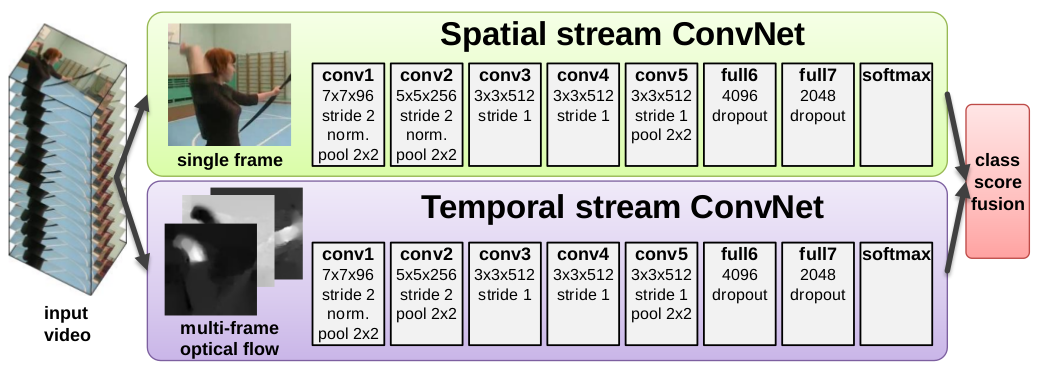
\includegraphics[width=0.9\textwidth]{img_deep/twostream_architecture}
    \caption{Two-stream architecture for video classification, depicting the spatial- and temporal-stream with implementation details as deep Convolutional Neural Network \cite{simonyan_two-stream_2014}}
    \label{fig:twostream_architecture}
\end{figure}

Spatial stream: Takes single video frames as input. Performs action recognition from still images and is fairly competitive on its own. Basically an image recognition architecture. Advantage: Can be pre-trained using large amount of image data, here from the ImageNet challenge dataset cite (??).

Spatial part of a video, i.e. the individual static frames, convey information about the objects and persons in the scene.

Temporal stream: is trained to recognize actions from motions given in the form of dense optical flow.

The temporal part of a video, i.e. the change between frames, conveys information about the movement of the observer (camera) and the movement of objects in the scene.

The second normalisation layer was removed from the the temporal stream network in order to reduce memory usage.

The authors propose two methods for constructing the input to the temporal network by stacking optical flow displacement fields along several consecutive frames of the input video.

\textbf{Optical Flow Stacking:} \\
A dense optical flow field $\mathbf{d}_t(u,v)$ of two consecutive frames at times $t$ and $t+1$ can be thought of as a two dimensional vector-field, which maps the displacement of each pixel along the transition from frame $t$ to $t+1$. In this case $u,v \in \mathbb{N}$, $1 \leq u \leq w$ and $1 \leq v \leq h$ where $w$ and $h$ are the width and height of the video frames.

The horizontal and vertical components $d_t^x(u,v)$, $d_t^y(u,v)$ can be interpreted as image channels.

This method constructs the input volume $I_\tau \in \mathbb{R}^{w \times h \times 2L}$ of the temporal stream network by stacking the horizontal and vertical components of the dense optical flow field along $L$ consecutive frames, beginning at time $\tau$. Formally, with $1 \leq k \leq L$:
\begin{align*}
    I_\tau(u,v,2k-1) = d_{\tau + k - 1}^x(u,v) \\
    I_\tau(u,v,2k) = d_{\tau + k - 1}^{y}(u,v)
\end{align*}

\textbf{Trajectory Stacking:} \\
Instead of sampling at fixed locations in each frame, this methods samples the dense optical flow field along the motion trajectories of the initial points in frame $\tau$.

Let $\mathbf{p}_k$ denote the motion trajectory of initial point $(u,v)$. With $1 < k \leq L$ and \mbox{$\mathbf{p}_1 = (u,v)$} the trajectory is recursively defined by:
\begin{align*}
    \mathbf{p}_k = \mathbf{p}_{k-1} + \mathbf{d}_{\tau + k - 2}(\mathbf{p}_{k-1})
\end{align*}

The input volume can then be constructed by sampling the horizontal and vertical optical flow components along these trajectories.

\begin{align*}
    I_\tau(u,v,2k-1) = d_{\tau + k - 1}^x(\mathbf{p}_{k}) \\
    I_\tau(u,v,2k) = d_{\tau + k - 1}^y(\mathbf{p}_{k})
\end{align*}

\begin{figure}[H]
    \centering
    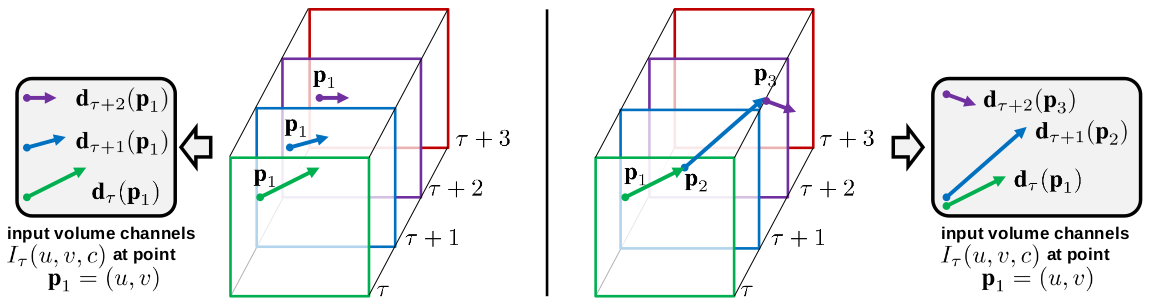
\includegraphics[width=0.9\textwidth]{img_deep/trajectory_stacking}
    \caption{Construction of input volumes from multi-frame optical flow. Left: Optical Flow Stacking. Right: Trajectory Stacking \cite{simonyan_two-stream_2014}}
    \label{fig:trajectory_stacking}
\end{figure}

Since the Convolutional Networks require fixed sized inputs, the authors sample a $224 \times 224 \times 2L$ subvolume from $I_\tau \in \mathbb{R}^{w \times h \times 2L}$ and use it as the temporal networks input.

By using optical flow, the authors explicitly incorporate a representation of motion in their action recognition architecture.

The authors further describe two optional techniques that are evaluated for constructing the inputs with either one of optical flow stacking methods.
\begin{enumerate}
    \item \textbf{Bi-directional Optical Flow}: The input volume $I_{\tau}$ is created by using regular forward optical flow from frame $\tau$ to $\tau + L/2$ and additionally calculated optical flow from frame $\tau$ to $\tau - L/2$ in the backwards direction. Stacking the horizontal and vertical components of these optical flow fields results in an input volume of length $L/2$ around frame $\tau$ in both directions. 
    \item \textbf{Mean flow subtraction}: The displacement vectors between two frames can dominantly be caused by global movement of the camera. Compared to regular camera-motion compensation, the authors use a simpler approach and just subtract the mean vector from each displacement field $\mathbf{d}_t$.
\end{enumerate}

An advantage of separating the spatial and the temporal stream is the possibility of pre-training the spatial net with large pre-existing image datasets (here ImageNet ILSVRC-2012 ??).

For training the temporal stream network with video-data, the authors address the general problem of video action recognition, that the existing datasets are too small in comparison to their image-dataset counterparts.

The authors use, according to the multi-task learning paradigm \cite{collobert_unified_2008}, the UCF-101 and the HMDB-51 dataset simultaneously for training the temporal stream network (see chapter ??). 

By training a network on several tasks (here UCF-101 classification and HMDB-51 classification), the network learns more general video representations, since the second task acts as regulariser and more data can be utilized.

The authors implement this by using two softmax classification layers, one for each dataset. Each softmax layer has its own loss function and the sum of the individual losses is taken as the overall training loss for computing the weight updates by backpropagation.

Training for both networks is conducted with mini-batch gradient descent with 256 randomly selected videos at each iteration. From each of those videos, a single frame is randomly chosen, a $224 \times 224$ sub-image is randomly cropped, randomly horizontal flipped, RGB jittered and then used as training input for the spatial stream network.

An optical flow volume is constructed for this selected frame as described above. For optical flow computation the authors use a fast implementation (0.06s per pair of frames) from the OpenCV toolbox. Despite it's speed, on-the-fly computation of optical-flow would be a bottleneck and is therefore pre-computed and stored for the complete datasets.

The creators of UCF-101 and HMDB-51 provide three splits of their datasets into training- and testing-data. The standard evaluation procedure is to report the average accuracy over those three splits, which the authors follow in this work as well.

The authors build their final design of the two-stream architecture by evaluating different setups for the spatial and temporal stream network on their own using UCF-101 (split 1).

Besides using two different dropout rate (0.5 and 0.9), the performance of the spatial-stream network is evaluated for:
\begin{enumerate}
    \item Training the complete network from scratch on UCF-101.
    \item Pre-training the network on ILSVRC-2012 and fine-tuning it on UCF-101.
    \item Pre-training the network on ILSVRC-2012 and fine-tuning of only the last (classification) layer.
\end{enumerate}

For evaluating the temporal-stream network a fixed dropout rate of 0.9 is chosen, because the network needs to be trained from scratch. The performance is then measured for:
\begin{enumerate}
    \item Using one or several (stacked) optical flow displacement fields $L \in {1,5,10}$.
    \item Regular optical flow stacking
    \item Trajectory stacking
    \item Using bi-directional optical flow
    \item Using mean subtraction
\end{enumerate}

The findings are presented in table \ref{tab:twostream_archeval}.

Spatial-stream network: The authors decided on pre-trained the network on ILSVRC and fine-tuning only the last layer.

Temporal-stream network: Mean subtraction and stacking multiple optical flows is beneficial, so $L=10$ is used as the default setting. Regular optical flow stacking performs better than trajectory stacking and bi-directional optical flow only yields slight improvement against forward optical flow. Therefore regular forwars optical flow stacking is chosen for the temporal-stream network.

The authors highlight that the temporal-stream network significantly outperforms the spatial-stream network, which confirms the importance of motion information for action recognition from video.

\begin{table}[H]
    \centering
    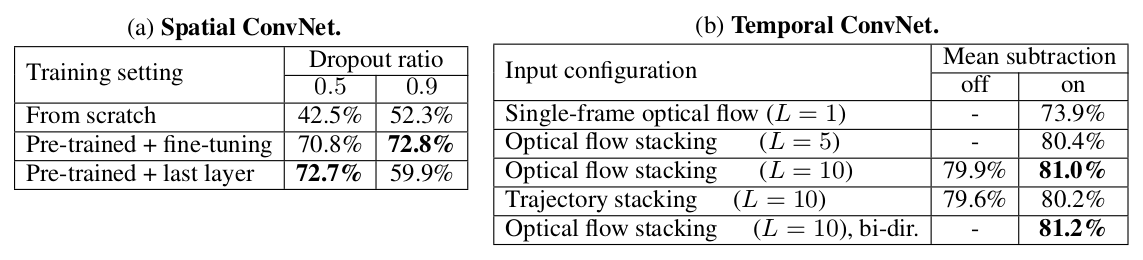
\includegraphics[width=\textwidth]{img_deep/twostream_archeval}
    \caption{Performance of the individual convolutional networks on UCF-101 (split 1) \cite{simonyan_two-stream_2014}}
    \label{tab:twostream_archeval}
\end{table}

After having found the optimal configurations for the individual temporal-stream and spatial-stream networks, the authors evaluate different fusion methods (averaging and SVM) and find that fusion by SVM performs best. The fused network's performance significantly improves over the individual network's performance, which implies, that the spatial and temporal recognition stream are complementary.

\begin{table}[H]
    \centering
    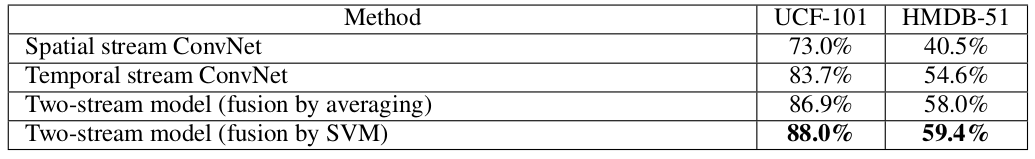
\includegraphics[width=\textwidth]{img_deep/twostream_results}
    \caption{Mean accuracy over three splits on UCF-101 and HMDB-51 \cite{simonyan_two-stream_2014}}
    \label{tab:twostream_results}
\end{table}

The results in table \ref{tab:twostream_results} show, that fusion by SVM works best.

\subsubsection{Action recognition with trajectory-pooled deep-convolutional descriptors -- Wang et al. (2014)}

\subsubsection{Fusing Multi-Stream Deep Networks for Video Classification -- Wu et al. (2015)}

\subsubsection{Towards good practices for very deep two-stream convnets -- Wang et al. (2015)}

\subsection{Recurrent Models}

\subsection{Generative Models}
Restricted Boltzmann Machine

\subsection{Temporal Coherency Networks}
